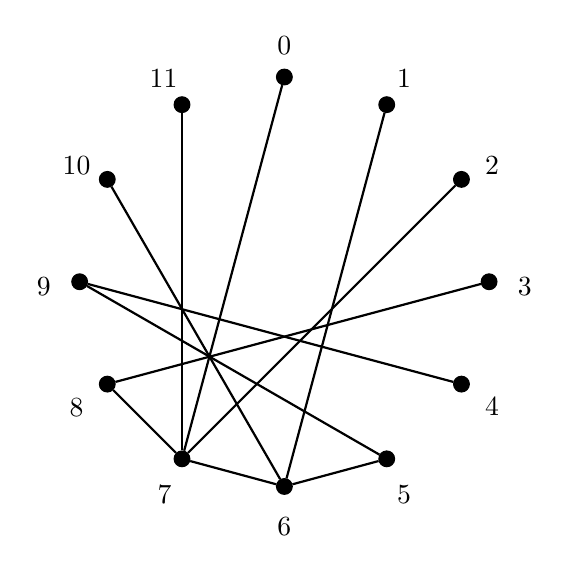
\begin{tikzpicture}
	\tikzset{enclosed/.style={draw, circle, inner sep=0pt, minimum size=0.2cm, fill=black}}

	\node[enclosed, label={above, xshift=0cm, yshift=0.052cm:0}] at (3.38, 5.2)(0){};
	\node[enclosed, label={above, xshift=0.221cm, yshift=-0.013cm:1}] at (4.68, 4.849)(1){};
	\node[enclosed, label={above, xshift=0.39cm, yshift=-0.169cm:2}] at (5.629, 3.9)(2){};
	\node[enclosed, label={above, xshift=0.455cm, yshift=-0.403cm:3}] at (5.98, 2.6)(3){};
	\node[enclosed, label={above, xshift=0.39cm, yshift=-0.624cm:4}] at (5.629, 1.3)(4){};
	\node[enclosed, label={above, xshift=0.221cm, yshift=-0.793cm:5}] at (4.68, 0.351)(5){};
	\node[enclosed, label={above, xshift=0cm, yshift=-0.858cm:6}] at (3.38, 0)(6){};
	\node[enclosed, label={above, xshift=-0.221cm, yshift=-0.793cm:7}] at (2.08, 0.351)(7){};
	\node[enclosed, label={above, xshift=-0.39cm, yshift=-0.637cm:8}] at (1.131, 1.3)(8){};
	\node[enclosed, label={above, xshift=-0.455cm, yshift=-0.403cm:9}] at (0.78, 2.6)(9){};
	\node[enclosed, label={above, xshift=-0.39cm, yshift=-0.169cm:10}] at (1.131, 3.9)(10){};
	\node[enclosed, label={above, xshift=-0.234cm, yshift=-0.013cm:11}] at (2.08, 4.849)(11){};
	\draw [thick] (0)--(7);
	\draw [thick] (5)--(9);
	\draw [thick] (6)--(1);
	\draw [thick] (6)--(5);
	\draw [thick] (6)--(10);
	\draw [thick] (7)--(2);
	\draw [thick] (7)--(6);
	\draw [thick] (7)--(8);
	\draw [thick] (7)--(11);
	\draw [thick] (8)--(3);
	\draw [thick] (9)--(4);
\end{tikzpicture}

